\documentclass[review]{elsarticle}

\usepackage{lineno,hyperref,booktabs,multirow,cleveref,pdflscape}
\modulolinenumbers[5]

\journal{Environmental Software and Modeling}

\bibliographystyle{APA-style}\biboptions{authoryear}

\begin{document}

\begin{frontmatter}

\title{Resource Alignment Service and Its Application in Envisioning the Model Web}

\author[address]{Peishi Jiang}
\author[address]{Mostafa Elag}
\author[address]{Praveen Kumar\corref{correspondingauthor}}

\cortext[correspondingauthor]{Corresponding author}
\ead{kumar1@illinois.edu}

\address[address]{Ven Te Chow, Hydrosystem Laboratory, Civil and Environmental Engineering, University of Illinois, Urbana, USA}

\begin{abstract}
Development of integrated Geoscience system increasingly requires the coupling multidisciplinary models and integration between data and models. Many Geoscience communities have adopted an approach of disseminating their models over the web, which are known as Model as a Service (MaaS). The web serviced models can be easily (re)used, accessed, and extended. Furthermore, the concept of Model Web has been recently proposed to describe a service-oriented architecture in coupling web serviced models. To envision a world of Model Web, one of the key challenges is to ensure the semantic interoperability of serviced models. To address this need, we put forward Semantically-Enabled Modles (SEM) where the information of a web serviced model is enriched by adding a semantic layer on the model, and designed the Resource Alignment Service (RAS) to ensure the semantic consistency between information exchanged between SEMs. In this paper, we first present the designs of SEM and RAS, and then demonstrate RAS application for both semantic coupling serviced models and integration of serviced models and data. A workflow of heterogeneous collection of web serviced data and models is created. Finally, we show how the semantic interoperability issue in coupling SEMs can be solved by utilizing RAS.
\end{abstract}

\begin{keyword}
Model Web \sep Semantic Interoperability \sep Resource Alignment Service (RAS) \sep Semantically-Enabled Model (SEM) 
\end{keyword}

\end{frontmatter}

\linenumbers

\section{Introduction}For decades, integrated environmental modeling has been applied in investigating the mechanism of the entire ecosystem, which becomes increasingly complex under climate change and human impact recently \citep{argent2004, laniak2013}. With the growing efforts in integrated modeling, scientists with a solo discipline background are able to access, reuse and couple resources (i.e., models and data) from various disciplines. It therefore enhances their assessment, prediction and management abilities of a complicated natural system. One of the approaches is through envisioning a world of “Model Web”, where the functionalities of models are exposed through web services and these resources are integrated via the internet \citep{geller2007, geller2008, nativi2013}. Hence, one of the challenges facing the community is to achieve the “minimal barriers to entry” \citep{nativi2013} or the interoperability between the serviced resources. In this study, we aim to propose a mechanism ensuring the semantic consistency of information flowing among serviced-oriented modeling.

The application of service-oriented architecture in environmental modeling just starts recently \citep{castronova2013, mineter2003, granell2010, goodall2011, goodall2013}. Following the concept of Software as a Service (SaaS), models and data can also be exposed as web services, called as Model as a Service (MaaS) and Data as a Service (DaaS), respectively. MaaS or DaaS are able to exchange data with other serviced models over the web, implying a loose-coupling approach of model integration \citep{goodall2011}. It is different from the traditional integrated modeling approach through tight coupling, where the initial independent models are coupled under a modeling integration application or framework. The representative integration frameworks include the Community Surface Dynamics Modeling System (CSDMS), Earth System Modeling Framework (ESMF), OpenMI standard and so forth \citep{hill2004, peckham2013, moore2005}. The advantage of the tight-coupling approach is that the framework entirely controls both the data structures and processes of all parts of the model. Nevertheless, due to the fixed convention or standard of a framework, it is difficult to couple models not following the standard or conventions. On the contrary, through the service-oriented loose-coupling approach, only the uniform protocol of data exchanging is required \citep{goodall2011}. It allows individual model developers or groups to maintain and update their models conveniently.

To achieve a world of interoperable serviced models and data, the concept of “Model Web” was put forward by \citep{geller2008}. Later, Nativi explicitly defined it as “a dynamic web of models, integrated with databases and websites, to form a consultative infrastructure where researches, managers, policy makers, and the general public can go to gain insight into ‘what if’ questions” in initiating it under the project of the Group on Earth Observation” \citep{nativi2013}. Several efforts have been made to draw the picture of “Model Web”. \citet{goodall2011} exposed water resource models as web services through Web Processing Service (WPS) and demonstrated how it could be encapsulated as OpenMI-compliant models. Then, they furthered the idea of servicing an OpenMI-compliant model based on WPS by considering the case of time-dependent models \citep{castronova2013}. Furthermore, an OpenMI-ESMF web service wrapper was developed to couple a climate model implemented via ESMF web service with an OpenMI-compliant hydrologic model running on a personal computer \citep{goodall2013}.\\
One of the key technical challenges in envisioning “Model Web” is to achieve the “minimal interoperability agreement” between serviced resources \citep{nativi2013}. It requires both a uniform protocol for communication and the semantic consistency of quantities exchanging between services.

Without it, semantics is one of the impediments to consumption and reuse of online heterogeneous or long-tail resources \citep{elag2015} as shown in Figure \ref{figure1}. The semantic consistency requirements include: (1) semantic mediation between variable names; (2) conversion of mismatched units; (3) temporal alignment of resource time horizon and (4) spatial alignment of resources spatial attributes. The existing efforts described in the previous paragraph try to achieve such interoperability by applying a specific standard. For instance, apply OpenMI standard in integrating water resource models serviced by WPS \citep{goodall2011, castronova2013}. Nevertheless, the application of a certain standard or framework might not be fruitful. This is because the existence of different standards or frameworks in different domains might imply the adoption of a specific framework in one discipline, thus complicating the online communication of serviced resources from various disciplines. For example, an OpenMI-compliant serviced model cannot talk with a serviced model embedded in Object Modeling System (OMS, \cite{david2013}) without a proper wrapper for communication between OpenMI and OMS. Furthermore, standards like OpenMI do not allow semantic mediation between variable names, prohibiting the integration of models with variables in alias names.

\begin{figure}[!htbp]
\centering
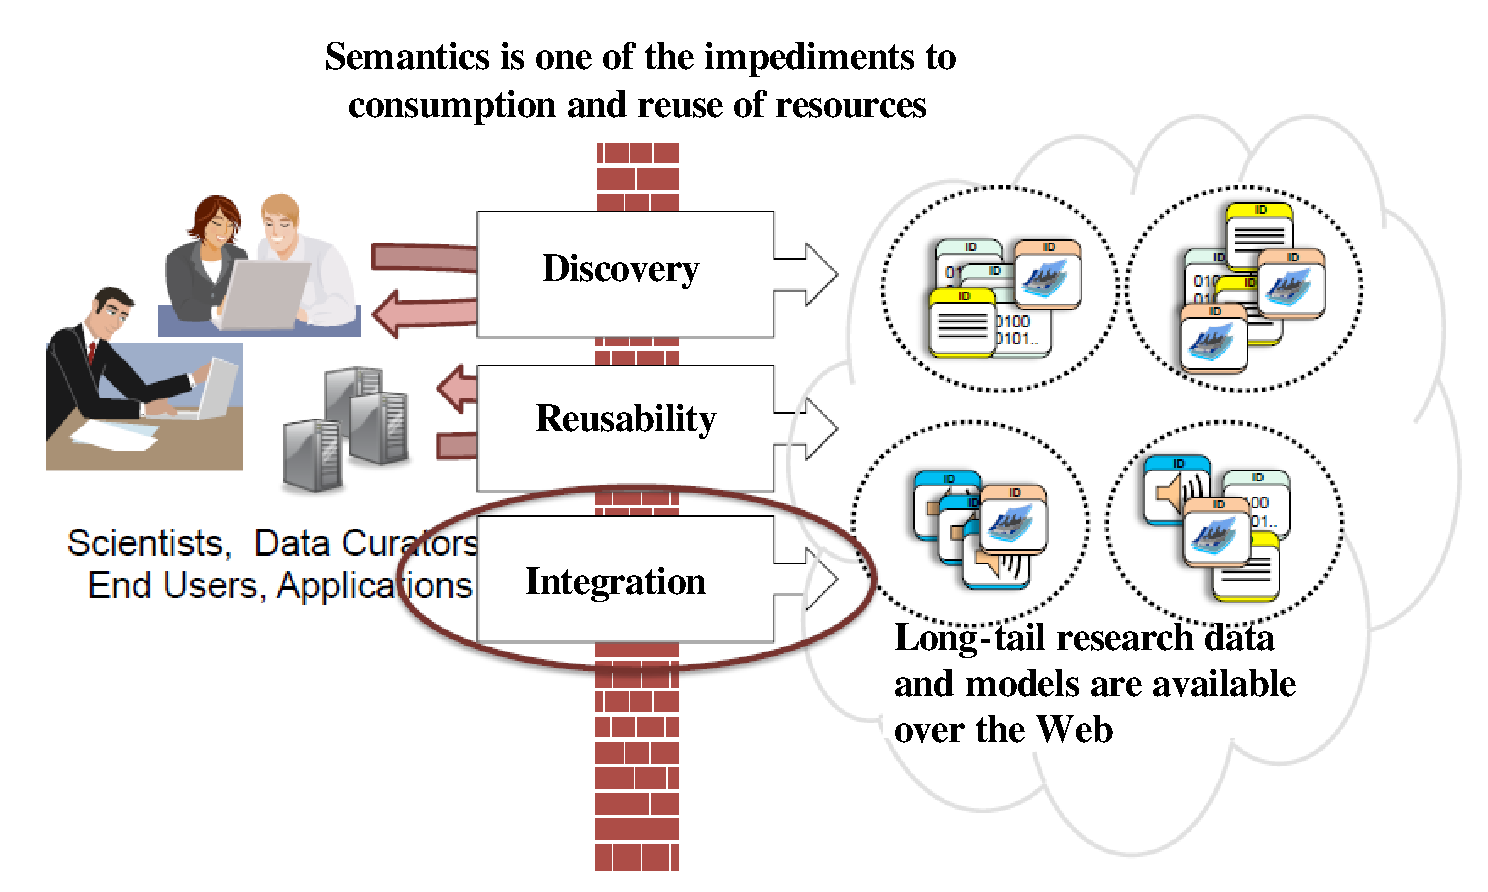
\includegraphics[scale=0.5]{../figures/figure_1.eps}
\label{figure1}
\caption{Semantics as the impediments for scientists, data consumers and web applications to integrating heterogeneous or long-tail resources over the web.}
\end{figure}

To tackle the issue of semantic interoperability of integrating service-oriented modeling, we introduce the Semantically-Enabled Model (SEM) by adding a semantic layer on top of a serviced model or MaaS, and then utilize a Web service named Resource Alignment Service (RAS) to align the quantities exchanging between SEM over the web. As a product of GeoSemantic framework, which aims to overcome the semantic heterogeneity among long-tail models an data collections \citep{elag2015}, RAS is designed as a metadata-agnostic Web service for the geoscience communities in order to ensure the semantic consistency of information transferred between serviced resources via the internet in terms of the name, unit, and temporal and spatial properties of variable.

In the remainder of the paper, Section 2 describes the general idea and the main components of GeoSemantic framework and the roles of SEMand RAS playing in it. In Section 3, the entire architecture of achieving the semantic interoperability in coupling serviced models is presented, including the designs of both SEM and RAS. Section 4 demonstrates the application of RAS in coupling SEMs and integration of SEM and data. First we create a workflow of heterogeneous collection of data and SEM. Then, we show how RAS can seamlessly align the semantics of quantities exchanging between these resources. Finally, a brief summary is given in Section 5, with mentions on the future work. 

\section{GeoSemantic Framework}GeoSemantic framework is an ongoing project that aims to allow the structured information seamlessly exchanging between various resources by achieving their semantic interoperability \citep{elag2015}. Through semantic web technology \citep{berners2001}, GeoSemantic enhances the capability of finding resources by searching a standard names graph, discovering the implicit relationships between resources by reasoning, and annotating a new or an existing resource by adding semantic tags.

As shown in Figure \ref{figure2}, to enable the search, annotation and discovery capability described above, a standard names graph is set up in a Jena TDB \footnote{https://jena.apache.org/documentation/tdb/} triple store,  to collect the linked vocabularies containing various standard names (SN), with four web services provided allowing users to fully utilize the functionality offered by GeoSemantic. The Knowledge Integration Service (KIS) imports the annotated standard names (e.g., CSDMS standard names \citep{peckham2014CSN}, the controlled vocabulary of observations data model \citep{horsburgh2009}, ingesting their thesaurus, and updates them into the GeoSemantics Wiki (a wiki describing the relationship between different standard names) and the triple store. The Knowledge Discovery Service (KDS) conducts semantic search and finds required resource in the triple store. The Semantic Annotation Service (SAS) annotates the metadata of resources in online repository (e.g., Clowder, an online resource collections developed under GeoSemantics framework). And the Resource Alignment Service (RAS) ensures the semantic consistency of information flowing between either serviced models (e.g., SEM) or a serviced model and serviced dataset (e.g.,  Clowder). In this study, we focus on the utilization of RAS on integration of SEMs to help envisioning the “Model Web”.

\begin{figure}[!htbp]
\centering
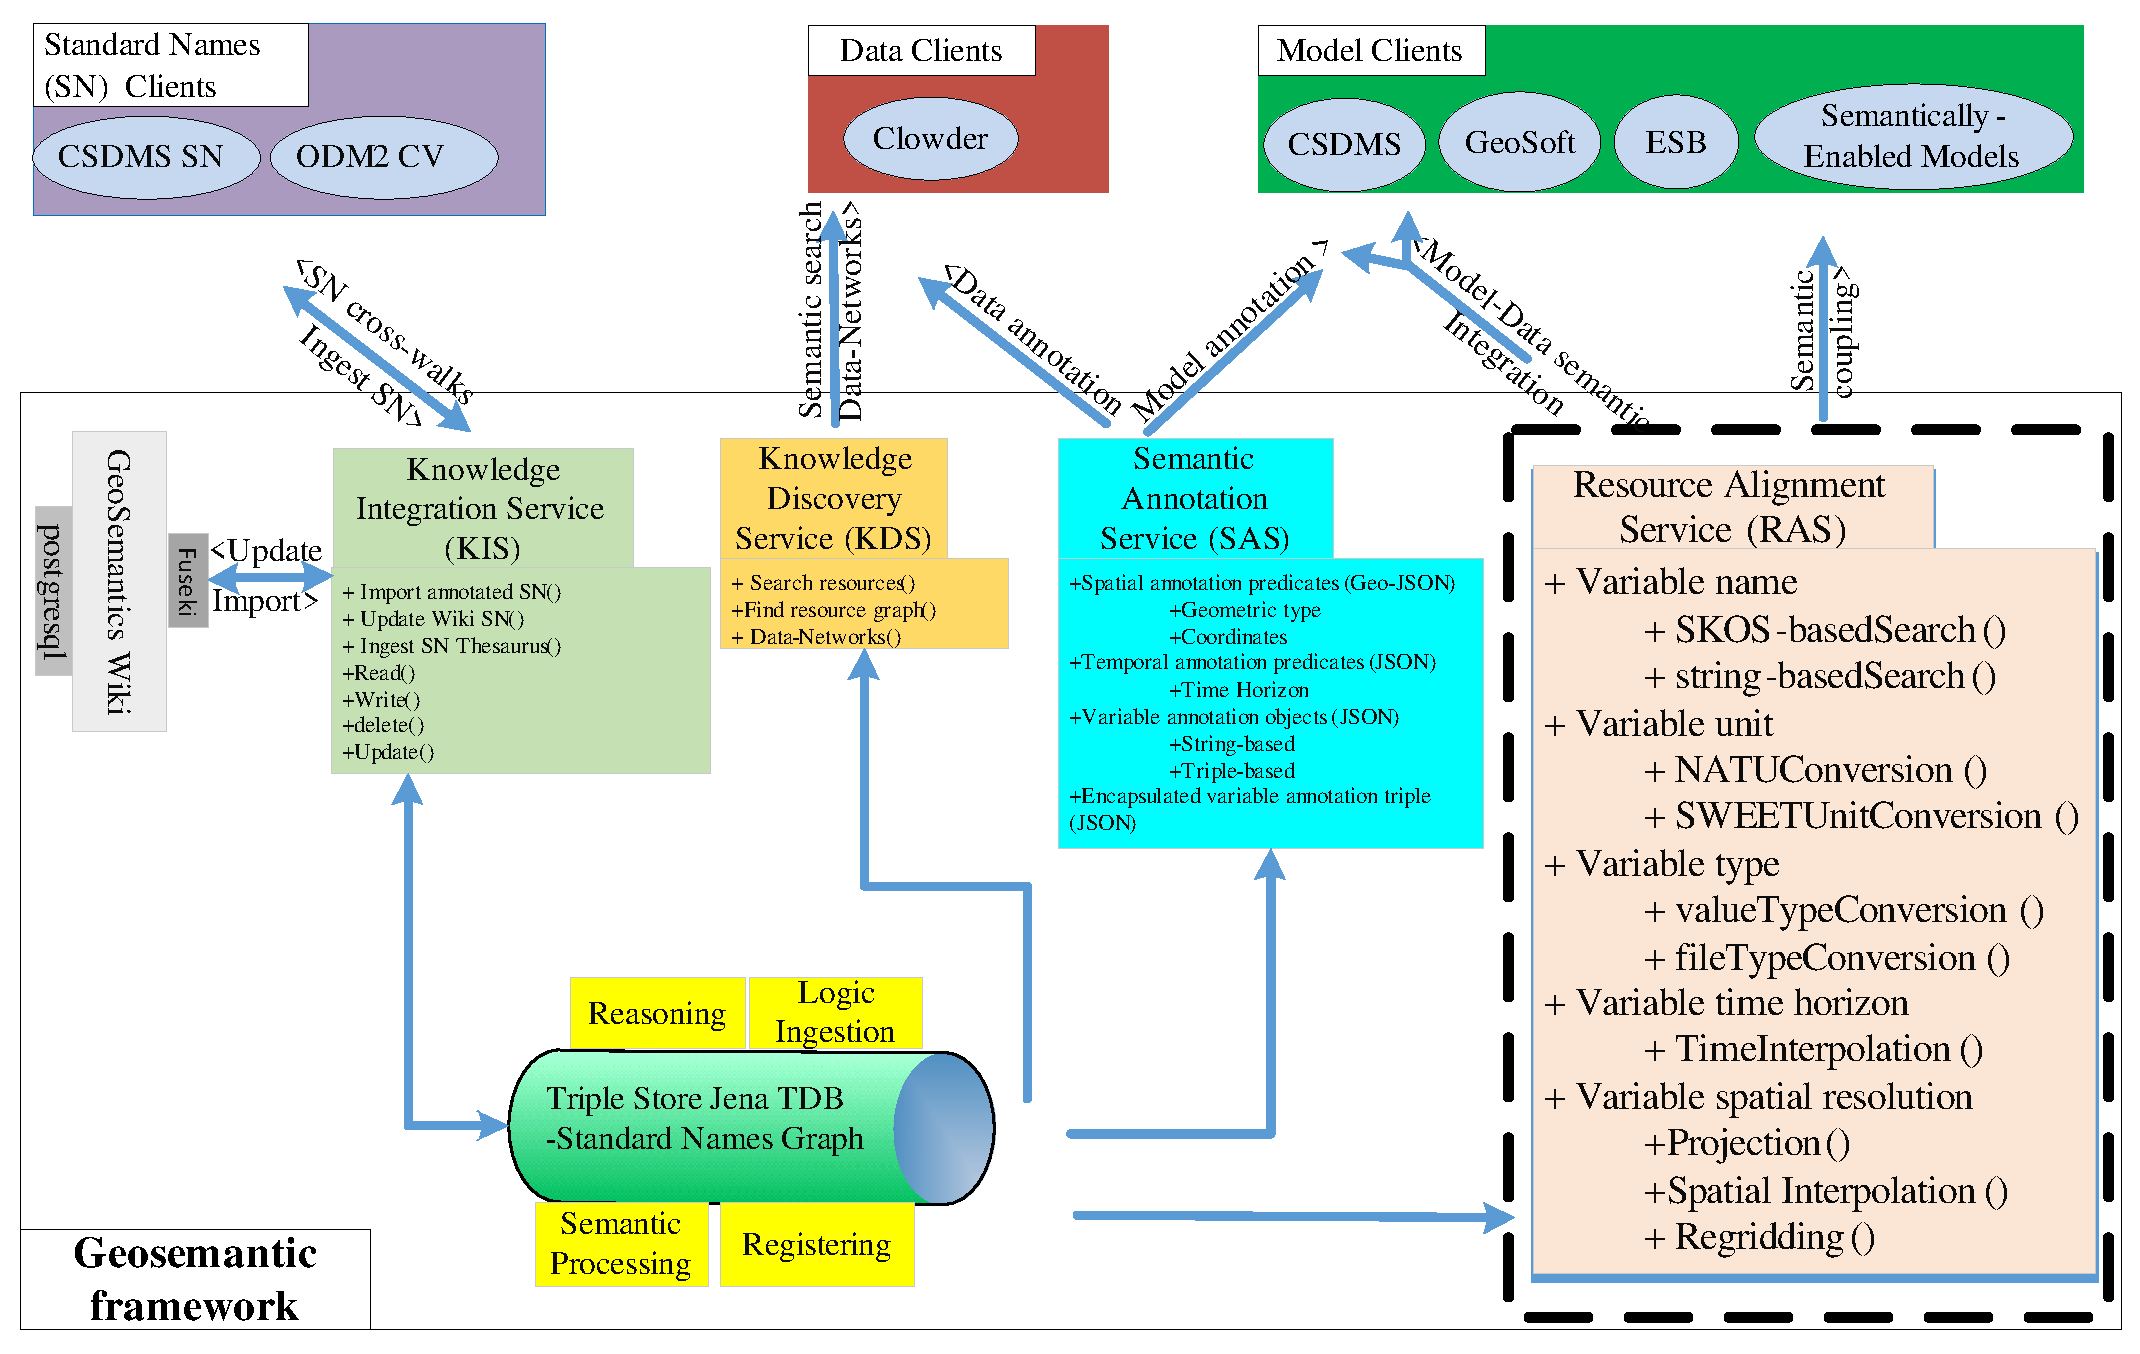
\includegraphics[scale=0.3]{../figures/figure_2}
\label{figure2}
\caption{The architecture of GeoSemantic framework. Four web services (i.e., KIS, KDS, SAS and RAS) are developed to allow users to import or ingest the standard names into the triple store, discover the inherent relationships between the resources from the triple store, annotate metadata of resources semantically and align two heterogeneous resources. In this study, we focus on the application of RAS in coupling SEM to envision the Model Web.}
\end{figure}

\section{Methodology}In this section, we present the architecture of how to ensure the semantic interoperability of serviced models as shown in Figure \ref{figure3}. To add a semantic layer on top of the available or new web serviced models, SEM is put forward by creating a dynamic metadata schema for processing these serviced models with minimum hum interventions. Then, RAS  is applied to ensure and do the required semantic alignment between the fields of the metadata schema of the relevant models in terms of (1) semantic mediation between variable names; (2) conversion of mismatched units; (3) conversion of different file types; (4) temporal alignment of resources time horizon; (5) spatial alignment of resources spatial attributes.

\begin{figure}[!htbp]
\centering
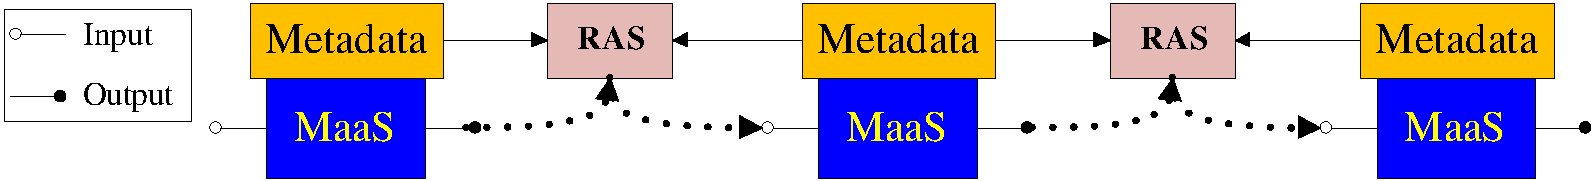
\includegraphics[scale=0.4]{../figures/figure_3}
\label{figure3}
\caption{The functionality of RAS in aligning the input and outputs of the serviced models.}
\end{figure}

\subsection{Semantically-Enabled Model(SEM)}The objective of SEM is to put a semantic layer on top of a serviced model to allow the external features of the model available and processable for other service like RAS. The models are exposed as services through the Open Geospatial Consortium (OGC) Web Processing Service (WPS). WPS is utilized because it provides a standard for processing data \citep{schut2007opengis}, which has proven to be successfully applied in other modeling study requiring data exchanging between services \citep{castronova2013, goodall2011, schaeffer2008,vitolo2012}.  

As depicted in the design of SEM in Figure \ref{figure4}, the semantic layer of SEM is added by creating a dynamic metadata schema based on a specified variable template in JSON format, which describes the name, the unit, the type, and the tempo-spatial properties of variable. The JSON-based metadata of a web serviced model includes not only the inputs and outputs but also the Uniform Resource Identifier (URI) for model execution. The metadata is assumed to live with the model codes in a same remote server and be serviced as well. It means the metadata of SEM is also available through an HTTP GET, with a different URI but the same namespace compared with the URI for the model execution through WPS.  

\begin{figure}[!htbp]
\centering
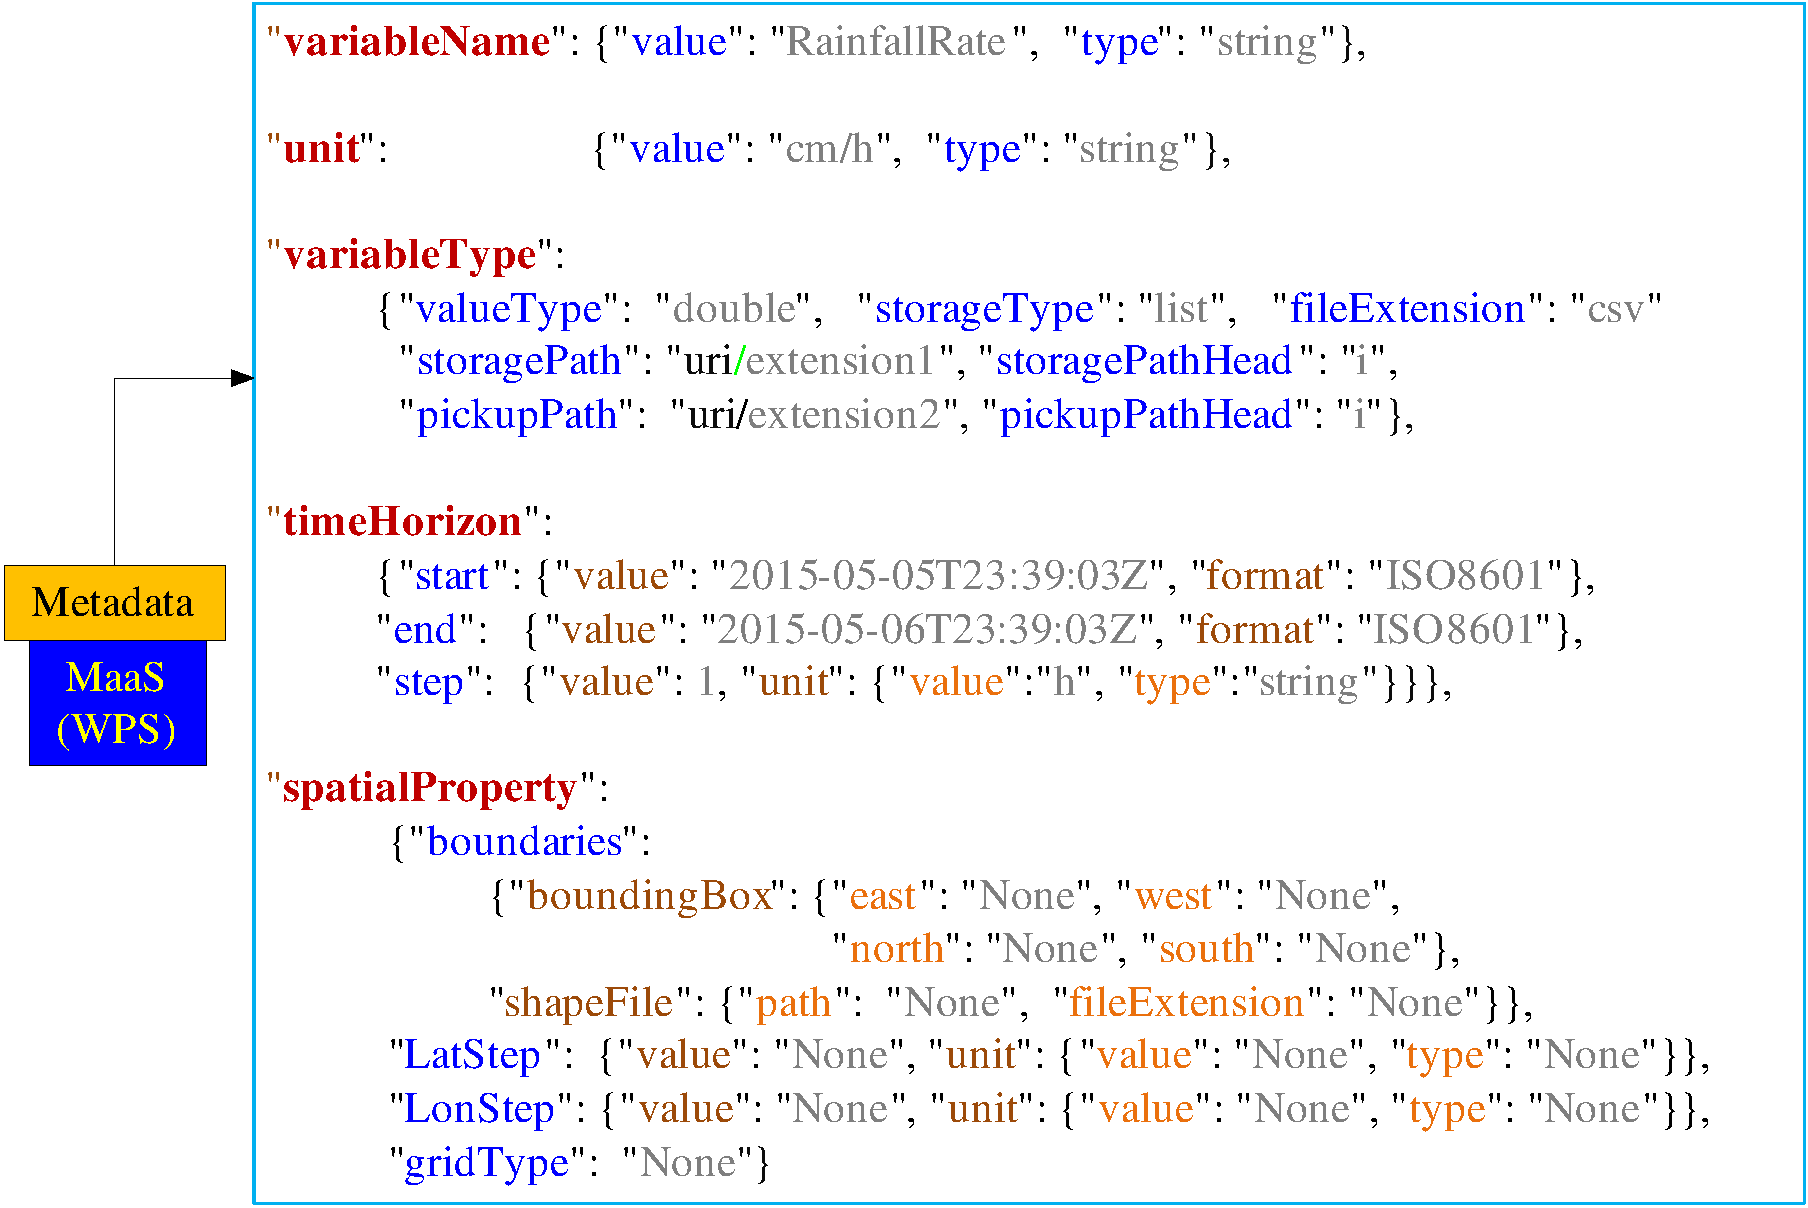
\includegraphics[scale=0.4]{../figures/figure_4}
\label{figure4}
\caption{Design of Semantically-Enabled Model (SEM) with a variable template example for \textit{Rainfall}.}
\end{figure}

To completely contain information of a variable used in a model, the basic elements of the JSON-based variable template include:

\paragraph{variableName} It illustrates the name of variable, with two keys: \textit{value} and \textit{type}. The field of type could be either “uri” or “string”, which indicates the field of \textit{value} as a URI or a simple string, respectively.

\paragraph{unit} It illustrates the unit of variable, with two keys: \textit{value} and \textit{type} functioning same as those of \textit{variableName}.

\paragraph{variableType} It illustrates the value, data and file type of variable in keys \textit{valueType}, \textit{storageType} and \textit{fileExtension}, respectively. The basic value types include integer, float, double, boolean, string and so forth. The field of storageType contains “singleValue” (a single value), “list” (a list of values) and “matrix” (a matrix of values). And the file type is detailed in \textit{fileExtension} (e.g., “.csv” for the Comma Separated Values (CSV) file, “.nc” for the Network Common Data Form (netCDF) file). Furthermore, to allow RAS be aware of where to store or pick up the data file, two other keys are added in \textit{variableType}: \textit{storagePath} and \textit{pickupPath}, with URIs as fields indicating the location of the file. Furthermore, \textit{storagePahHead} and \textit{pickupPathHead} indicate the headers of the data in the files with \textit{storagePath} and \textit{pickupPath}, respectively, if any.

\paragraph{timeHorizon} It illustrates the temporal property of variable, with keys: \textit{start}, \textit{end} and \textit{step}. \textit{start} and \textit{end} are the start and end time of variable used in the model. Both of them have two keys: \textit{value} and \textit{format}, where format indicates the format or standard (e.g., ISO8601) of the field of \textit{value}. If the start and end times are not required by the model, the fields of value of \textit{start} and \textit{end} are entered as “notSpecified”.  Moreover, \textit{step} describes the time step of variable, with information of time step value and time step unit (e.g., “h” for hour, “min” for minute) stored in keys \textit{value} and \textit{unit}.

\paragraph{spatialProperty} It illustrates the spatial property of variable, with keys: \textit{boundaries}, \textit{LatStep}, \textit{LonStep} and \textit{gridType}. \textit{boundaries} contains the boundaries of variable, stored either in a bounding box (with key \textit{boundingBox}) or a shape file (with key \textit{shapeFile}). The latitude and longitude resolutions of variable are depicted in \textit{LatStep} and \textit{LonStep} with keys \textit{value} and \textit{unit}. Finally, the type of grid (e.g., uniform, rectilinear) is described in \textit{gridType}.

It should be noted that if variable used in a model does not have any information for an attribute (key), the field of it is entered as “None”. For example, for a time series of rainfall at a specified location, the fields of all keys in \textit{spatialProperty} should be escaped as “None”.

\subsection{Resource Alignment Service (RAS)} RAS is developed as a service to ensure the semantic consistency of information exchanging between online resources. The entire functionality of it includes semantic mediation of variable names, conversion of mismatched units and file type, and tempo-spatial alignment. A Python web application package, Flask\footnote{http://flask.pocoo.org/}, is utilized to set up the service. In this study, it is applied to align quantities flowing between SEM.

\subsubsection{RAS Architecture}As shown in Figure \ref{figure5}, RAS is a web service allowing the alignment between two list variables in terms of: variable name, variable unit, variable value type, file type, variable temporal and spatial properties. The alignment is carried out for each pair of variables, say, aligning from variable I to variable II.

\begin{figure}[!htbp]
\centering
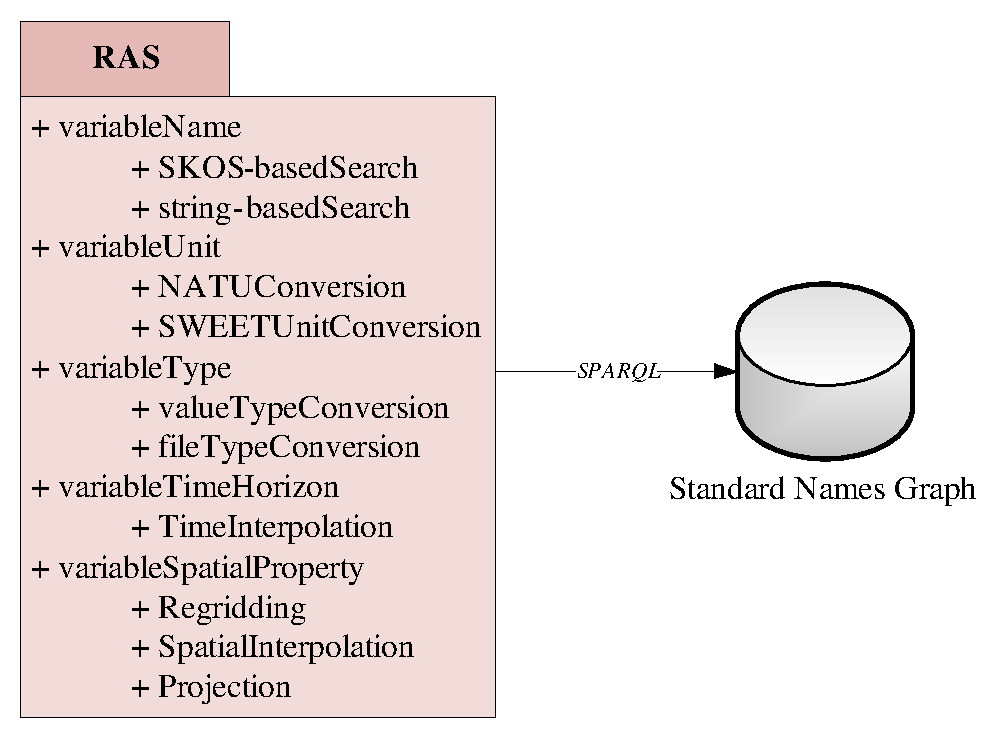
\includegraphics[scale=0.4]{../figures/figure_5}
\label{figure5}
\caption{The architecture of the Resource Alignment Service (RAS).}
\end{figure}

\paragraph{variable name} The semantic mediation of two variable names is conducted through either a SKOS-based search or a string-based search. SKOS-based search is applied for variable names in a form of URI. The procedures of it are (1) finding all the matched (i.e., \textit{skos:exactMatch} or \textit{skos:closeMatch}) variable names for variable I by querying the standard names graph through SPARQL\footnote{http://www.w3.org/TR/rdf-sparql-query/}, an Resource Description Framework (RDF) query language; (2) checking whether variable II is in the list of the matched variables of variable I (return matched if true). \textit{rdflib}\footnote{https://github.com/RDFLib/rdflib}, a Python library for working with RDF, is utilized for RDF querying. In addition, if the types of variable names are string, then the mediation is through string-based search. The variable name in string is first transformed in a URI format by assigning it with a model name space. Then SKOS-based search is used for semantic mediation. 

\paragraph{variable unit} Similar to the alignment of two variable names, the conversion of two variable units is based on \textit{natu} conversion and SWEET unit conversion, according to the types of units: string and URI, respectively. If the unit types are string, a Python unit conversion package, \textit{natu}\footnote{http://kdavies4.github.io/natu/} (Natural units in Python), is employed to perform the conversion. On the other hand, SWEET unit ontology is applied in the case that both the unit formats are URI. 

\paragraph{variable type} The alignment of the variable types of two variables is based on both the value and file types conversion. The value type alignment is straightforward through type conversion in Python (e.g., from \textit{float} to \textit{integer}). In terms of conversion in file types, currently the supported file types are csv/txt, xls and.nc, with the header information in the file if any. 

\paragraph{variable time horizon} The temporal property alignment of two variables is conducted through linear temporal interpolation, given the start time, the end time and the time step of each variable. By temporal interpolation approach, the actual time period of the data of variable II aligned from that of variable I is the intersection of the given time periods of the two variables. It means if the time periods (from the start time to the end time) of the two variables do not overlap, there is no data interpolated for variable II. 

\paragraph{variable spatial property} The alignment of two variables’ spatial property is carried out through regridding and projection. Based on the boundary and grid information of two variables, regridding is utilized for spatial interpolation from grids of variable I to those of variable II. Also, projection, or map projection is a transformation from the latitudes and longitudes of locations on earth of a sphere into grids or locations in a plane. This functionality is still under development.

\subsubsection{RAS Functionality} The purpose of RAS is to avoid the semantic mismatch of two variable lists by aligning each pair of variables through the functions described in Section 2.2.1. Generally, through HTTP POST method, the service takes the metadata of the two variables lists, along with the values of a list of variables, in JSON format. For example, to apply RAS to ensure that the output(s) of a SEM (say, SEM I) can be utilized as the input(s) of another SEM (say, SEM II), the following information is required to be fed into RAS: 
\begin{itemize}
\item the metadata of the output(s) of SEM I
\item the output values of SEM I
\item the metadata of the input(s) of SEM II
\end{itemize}
Then, the process of the semantic check and the alignment happens inside of the RAS service based on the alignment functions for the different properties (i.e., name, unit, type, time horizon and spatial property). In the case of alignment between input and output of two SEMs, the process is conducted based on the metadata of the two SEMs, which is introduced in Section 3.1. Once the alignment process finishes, the values of the other variable list, aligned from the provided values of the first list, is returned 262 in JSON format.

In addition, it should be noted that for each pair of variables, the alignment would fail in the cases of the following situations:
\begin{itemize}
\item the two variable names are mismatched through either SKOS-based or string-based search
\item the storage types of the two variables are not the same (e.g., one is a single value, another is a list of values).
\end{itemize}

\section{Application} Two applications are presented: (1) serviced data-model integration (DaaS $\rightarrow$ MaaS) and (2) serviced model-model integration (DaaS $\rightarrow$ MaaS $\rightarrow$ MaaS). All the MaaS are deployed as SEMs and RAS is utilized for ensuring the semantic interoperability between serviced resources.  In the first application, DaaS $\rightarrow$ MaaS, meteorological data stored Clowder is aligned to the format of the inputs of a SEM-based Priest-Taylor model through RAS. In the application of DaaS $\rightarrow$ MaaS $\rightarrow$ MaaS, RAS is used for the alignment between both the data from Clowder and the output of Priest-Taylor model and a SEM-based 1D Richard equation model. 

\subsection{DaaS and MaaS in Application} 
\subsubsection{SEMs in Application} The Priestley-Taylor approach is an approach for estimating evaporation at areas with low moisture stress, a modification of Penman’ approach for evaporation estimation \citep{priestley1972}. It requires information of net short wave and long wave radiation, ground heat flux and air temperature at a specific location. In this study, the ground heat flux is generated from a linear relationship between it and soil temperatures at different levels. 

Richards’ equation, developed by \cite{richards1931}, simulates the water movement process in unsaturated soils. Given the time series information of evaporation and precipitation, Richard’s equation is able to generate the profiles of both the soil pressure head and the soil moisture over time by solving its non-linear partial differential equation. In this study, 1D Richards equation is utilized in the application, which simplifies the whole process by considering the vertical direction. 

Both the models are serviced through PyWPS\footnote{http://pywps.wald.intevation.org/}, a Python implementation of WPS. The original codes of the two models are in Python and MATLAB for Priest-Taylor and 1D Richard equation, respectively. To allow the MATLAB-based 1D Richard equation model serviced by PyWPS, the package, MATLAB Engine for Python \footnote{http://www.mathworks.com/help/matlab/matlab-engine-for-python.html}, is used to enable calling MATLAB code from Python. Also, the JSON-based metadata of the two models, of which the example is provided in Figure \ref{figure4}, are also serviced and available through HTTP GET request, which is set up by Flask. 

\subsubsection{Clowder} In addition, Clowder, as a product of GeoSemantic framework, is developed as an online resource (i.e., model and data) repository allowing resource upload, annotation and extraction of the metadata of the resource. Users can annotate or extract the metadata of a resource through either a web page interface or web service APIs. The metadata available for annotation includes temporal/spatial reference, description, variable name mapping, abstract and so forth. To feed the required inputs of the two models, the soil surface temperature, the net short and long wave radiation, the air temperature, the precipitation and the soil temperature at depth of 4 meter in 2007 at Bondville are uploaded and annotated in Clowderas 306 shown in Figure \ref{figure6}.

\begin{landscape}
\begin{figure}[!htbp]
\centering
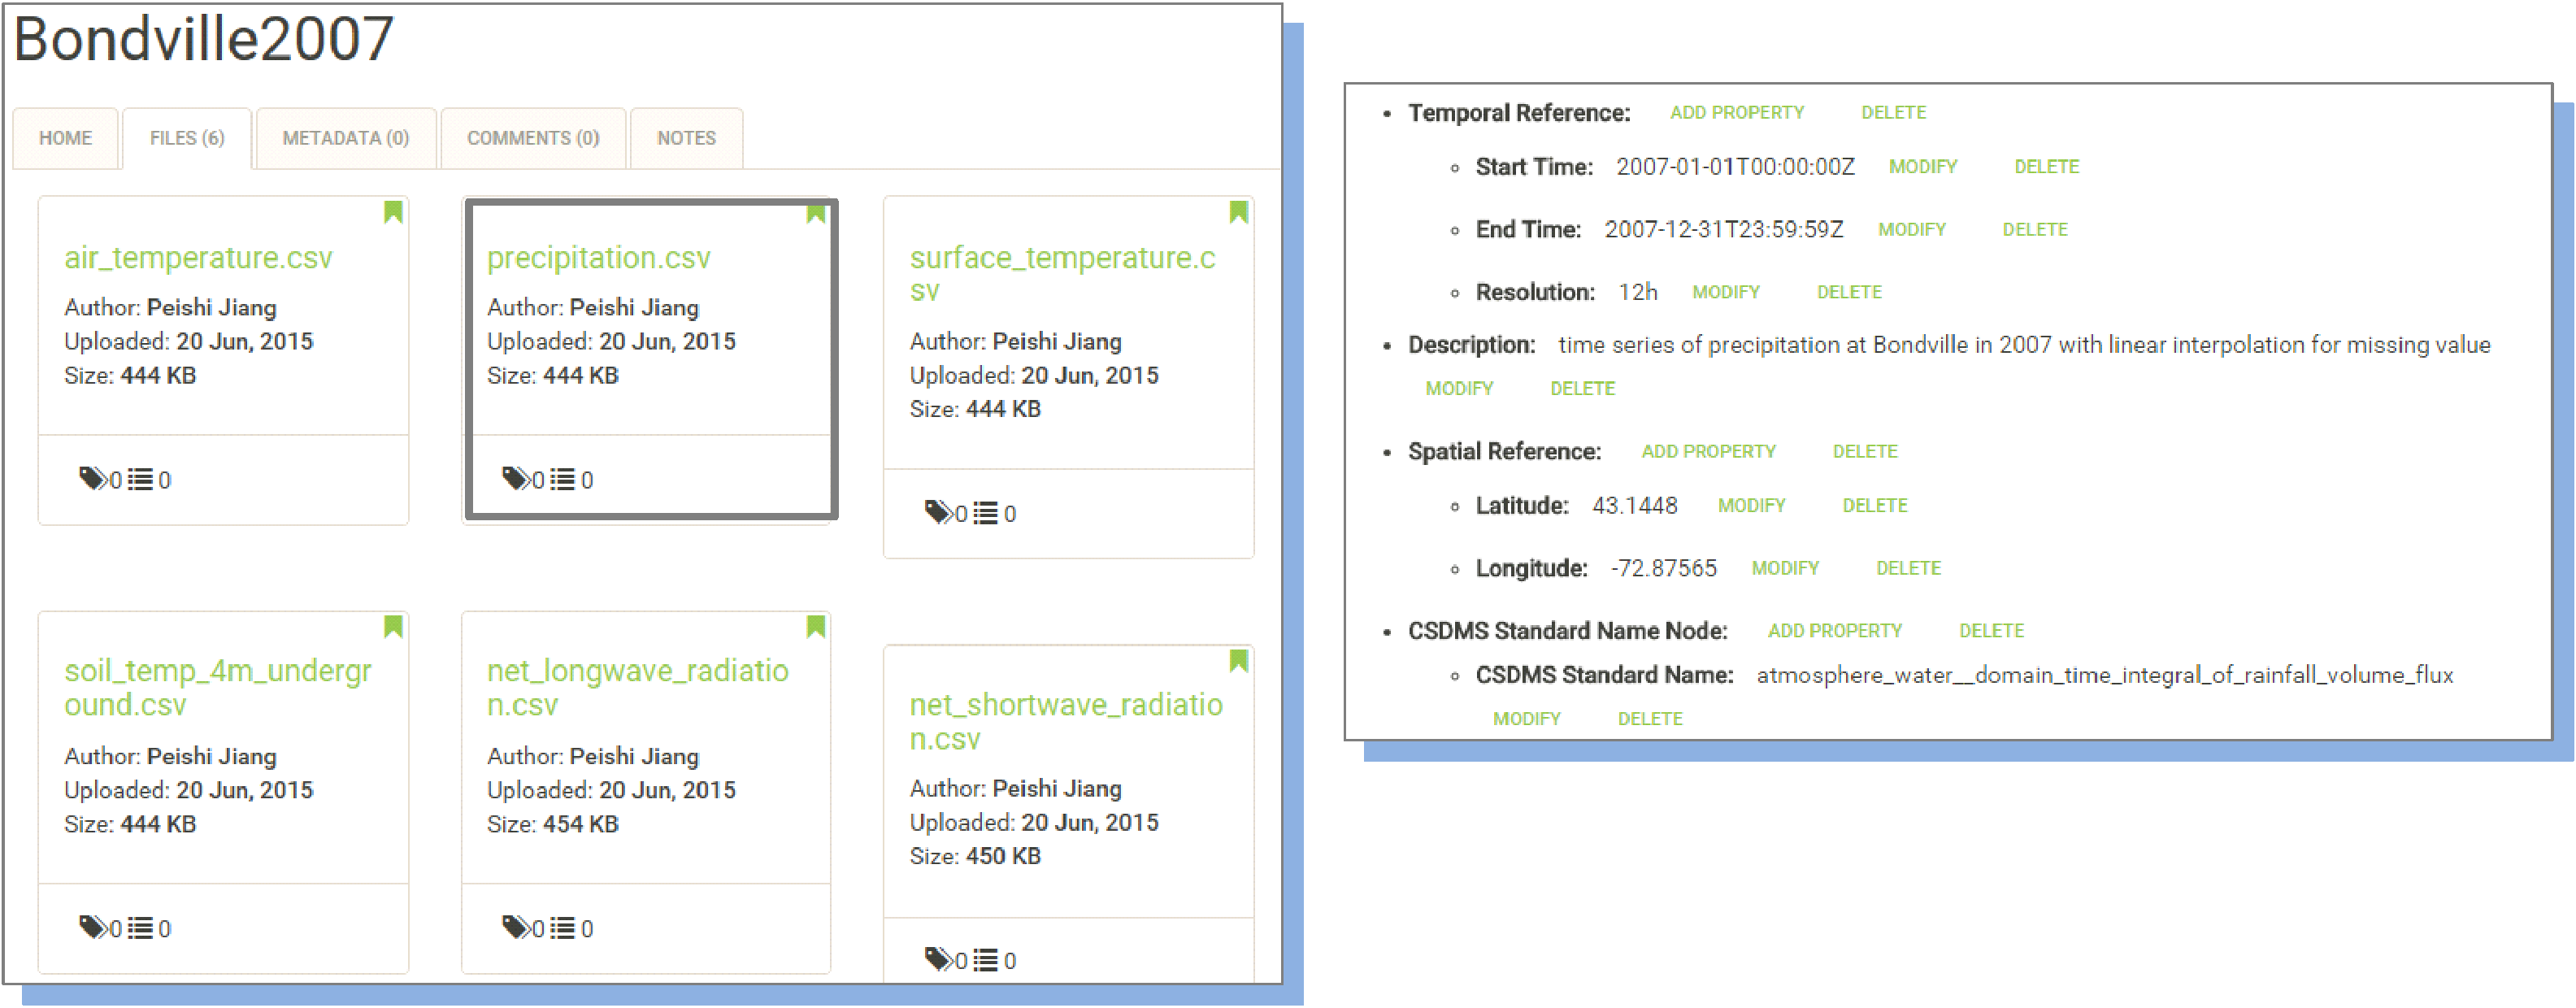
\includegraphics[scale=0.4]{../figures/figure_6}
\label{figure6}
\caption{The screenshots of the five environmental datasets at Bondville in 2007 uploaded to Clowder and the metadata of \textit{precipitation.csv} file.}
\end{figure}
\end{landscape}

\subsubsection{Relations and Heterogeneities among Data in Clowder and Variables in the two SEMs} Figure \ref{figure7} illustrates the relationships among the data stored in Clowder and the I/O of the two SEMs. In the first application (i.e., DaaS $\rightarrow$ MaaS), information stored in Clowder (i.e., the surface temperature, net long and short wave radiation, air temperature and soil temperature at depth of 4 meters at Bondville in 2007) is used for the input of the serviced Priest-Taylor model after a certain alignment through RAS. For the second application, the required inputs of 1D Richard equation are given by both the precipitation at Bondville in 2007 from Clowder and the evaporation output of the Priestley-Taylor model generated from the first application. 

\begin{figure}[!htbp]
\centering
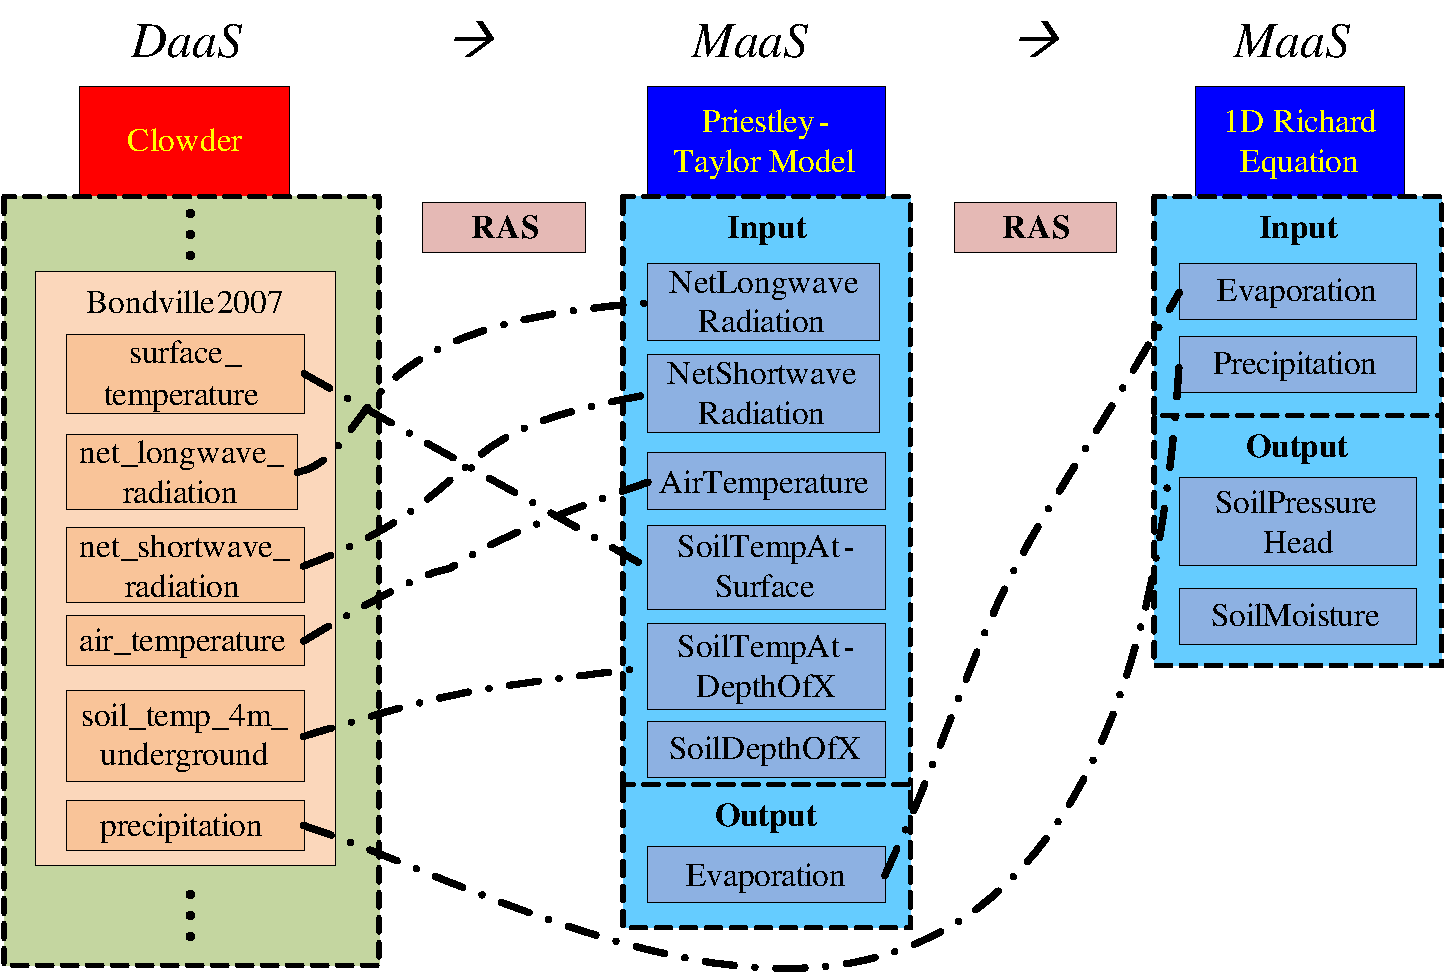
\includegraphics[scale=0.4]{../figures/figure_7}
\label{figure7}
\caption{The relationships among the Bonville’s environmental data in 2007 from Clowder and the inputs and outputs of Priestley-Taylor model and 1D Richard equation.}
\end{figure}

In both applications, RAS is utilized to ensure the semantic consistency of quantities flowing from either Clowder or the SEM’s output to the inputs of the twoSEMs. The semantic heterogeneities of the data used in Clowderand the I/O of the two models are provided in Table \ref{tabel1}. It can be observed that the variables or data differ from each other in terms of name, unit, value type, file extension and time horizon properties. In terms of naming, the names of data from Clowder are defined with an underscore separating words while variable names in the two models are in format of camelCase. Units and file extension of variables are also different. For example, the unit of data “precipitation” in Clowder is in mm while the required unit of the input “Rainfall” in 1D Richard equation is in cm; the format of Priestley-Taylor model’s output (“LandSurfaceEvaporation”) is netCDF but the “Evaporation” of 1D Richard equation requires CSV file. For time horizon, we assume that both the Priestley-Taylor model and 1D Richard equation has the same fixed time range but with different time steps as 1h and 0.5h, respectively. The fixed time range of the two models is for differing from the period of time of data from Clowder which covers the whole year 2007. 

\begin{landscape}
\begin{table}[h]
\small
\centering
\renewcommand{\arraystretch}{0.6}
\caption{The properties of the Clowder's data used in this study.}
\label{tabel1}
\begin{tabular}{*8c}
\toprule
Clowder&Name&Unit &Value type&File extension & Start time & End time & Time step                      \\
\midrule
\multirow{6}{*}{Data}&air\_temperature                      & degF        & double    & .csv  & 2007-01-01T00:00:00Z & 2007-12-31T23:59:59Z & 12h       \\
					    	      &surface\_temperature               & degF       & double    & .csv   & 2007-01-01T00:00:00Z & 2007-12-31T23:59:59Z & 12h       \\
							  &soil\_temp\_4m\_underground & degF        & double    & .csv  & 2007-01-01T00:00:00Z & 2007-12-31T23:59:59Z & 12h       \\
							  &net\_longwave\_radiation         & W*m-2     & double    & .csv   & 2007-01-01T00:00:00Z & 2007-12-31T23:59:59Z & 12h       \\
							  &net\_shortwave\_radiation       & W*m-2      & double    & .csv   & 2007-01-01T00:00:00Z & 2007-12-31T23:59:59Z & 12h       \\
							  &precipitation                             & mm           & double    & .csv   & 2007-01-01T00:00:00Z & 2007-12-31T23:59:59Z & 12h      \\
\midrule
Priestley-Taylor model&Name&Unit &Value type&File extension & Start time & End time & Time step                      \\
\midrule
\multirow{6}{*}{Input}&AirTemperature                     & degC     & double    & .csv   & 2007-05-01T00:00:00Z & 2007-08-31T23:59:59Z & 1h       \\
							  &NetLongwaveRadiation        & W*m-2   & double    & .csv   & 2007-05-01T00:00:00Z & 2007-08-31T23:59:59Z & 1h       \\
							  &NetShortwaveRadiation        & W*m-2  & double    & .csv   & 2007-05-01T00:00:00Z & 2007-08-31T23:59:59Z & 1h       \\
							  &SoilTempAtSurface               & degC     & double    & .csv   & 2007-05-01T00:00:00Z & 2007-08-31T23:59:59Z & 1h       \\
							  &SoilTempAtDepthOfXMeters & degC     & double    & .csv   & 2007-05-01T00:00:00Z & 2007-08-31T23:59:59Z & 1h       \\
							  &SoilDepthOfXMeters	           & m           & double    & /        & /								  & /								    & /      \\
Output                      &LandSurfaceEvaporation       & m           & double    & .nc     & 2007-05-01T00:00:00Z & 2007-08-31T23:59:59Z & 1h       \\
\midrule
1D Richard equation&Name&Unit &Value type&File extension & Start time & End time & Time step                      \\
\midrule
\multirow{6}{*}{Input}&AirTemperature                     & degC     & double    & .csv   & 2007-05-01T00:00:00Z & 2007-08-31T23:59:59Z & 1h       \\
							  &NetLongwaveRadiation        & W*m-2   & double    & .csv   & 2007-05-01T00:00:00Z & 2007-08-31T23:59:59Z & 1h       \\
							  &NetShortwaveRadiation        & W*m-2  & double    & .csv   & 2007-05-01T00:00:00Z & 2007-08-31T23:59:59Z & 1h       \\
							  &SoilTempAtSurface               & degC     & double    & .csv   & 2007-05-01T00:00:00Z & 2007-08-31T23:59:59Z & 1h       \\
							  &SoilTempAtDepthOfXMeters & degC     & double    & .csv   & 2007-05-01T00:00:00Z & 2007-08-31T23:59:59Z & 1h       \\
							  &SoilDepthOfXMeters	           & m           & double    & /        & /								  & /								    & /      \\
Output                      &LandSurfaceEvaporation       & m           & double    & .nc     & 2007-05-01T00:00:00Z & 2007-08-31T23:59:59Z & 1h       \\
\bottomrule
\end{tabular}
\end{table}
\end{landscape}

\subsection{Implementation} A workflow is created to carry out the coupling of heterogeneous data and models as presented in Figure \ref{figure7}. Basically, in the first application, based on the metadata of Priestley-Taylor model, data of \textit{air\_temperature}, \textit{surface\_temperature}, \textit{soil\_temperature\_underground}, \textit{net\_longwave\_radiation}  and \textit{net\_shortwave\_radiation} in Clowder is first aligned to the required semantics of the inputs of the Priestley-Taylor model by RAS. Then, once the input is ready, the model execution is conducted through a HTTP request to the WPS-based service. In the second application, RAS is used again to align from the output of Priestley-Taylor model and \textit{precipitation} data in Clowder to the two inputs of 1D Richard equation. The Richard equation execution is performed after the alignment.

To ensure the successful alignment through RAS, besides the utilization of the several conversion functions (e.g., unit conversion, temporal interpolation), a comprehensive standard names graph is also required for the semantic mediation of variable names. Figure \ref{figure8} shows how the variable names in Table \ref{tabel1} are related with each other by using SKOS. For example, \textit{AirTemperature} in Priestley-Taylor model is matched with \textit{air\_temperature} in Clowder based on their same \textit{skos:exactMatch} \textit{csn:atmosphere\_bottom\_air\_\_temperature}, a CSDMS standard name for describing air temperature at the bottom of the atmosphere.

\begin{landscape}
\begin{figure}[!htbp]
\centering
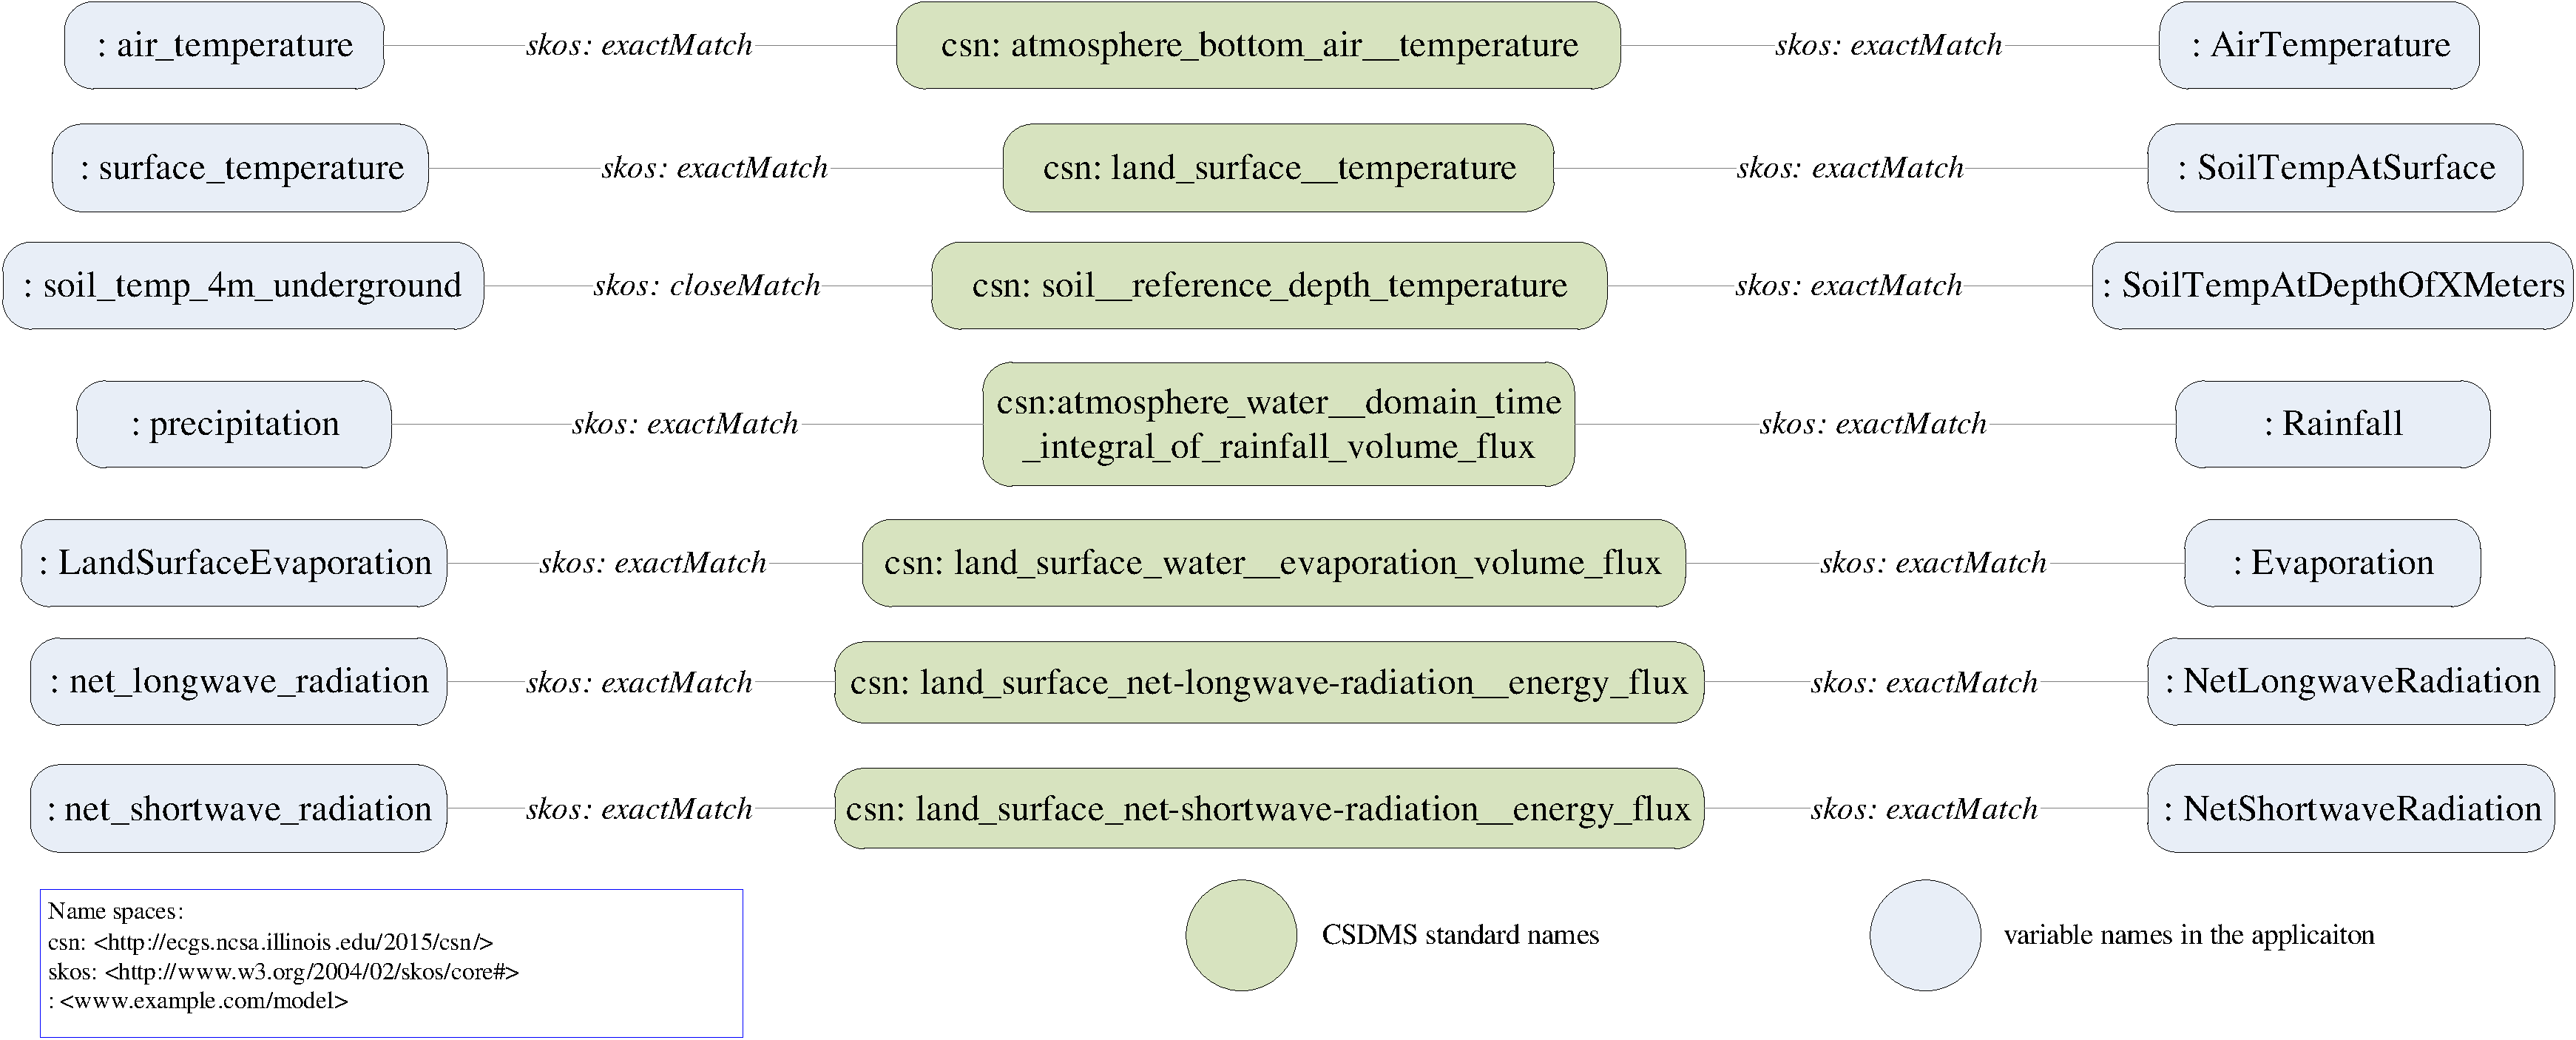
\includegraphics[scale=0.3]{../figures/figure_8}
\label{figure8}
\caption{The SKOS-based relationships between CSDMS standard names and the variable names in the application stored in the standard names graph.}
\end{figure}
\end{landscape}

\section{Summary and Future Work} An approach for ensuring the semantic consistency of information exchanging between serviced resources was designed to help integrating serviced models. To solve the semantic interoperability issue in envisioning a world of Model Web, serviced models or MaaS were semantically enabled as SEM with the application of the Resource Alignment Service (RAS) in dealing with the semantic inconsistency of quantities exchanging between SEMs. To allow the external features (e.g., inputs and outputs) of a model available for other clients (e.g., users or services), Semantically-Enabled Models (SEM) were put forward by adding semantic layer on top of a serviced model and the Open Geospatial Consortium’s (OGC) Web Processing Service (WPS) standard was utilized as the data specification. Based on the semantic information of SEM, RAS was then applied to check and resolve the misalignment of two lists of variables in terms of names, units, value and file types, temporal and spatial properties.  

A workflow of heterogeneous collection of serviced data and SEMs was created to show how RAS can seamlessly align the semantics of quantities exchanged between these resources. Priestley-Taylor model and 1D Richard equation were deployed as SEM serviced by PyWPS. Environmental data stored in Clowder was fed as inputs for the two models to create the workflow in a manner of DaaS $\rightarrow$ MaaS $\rightarrow$ MaaS as shown in Figure \ref{figure7}. The heterogeneities of data in Clowder and variables in the two models are presented in Table \ref{tabel1}. With the implementation shown in Section 4.2, we conclude that it is possible to resolve the semantic interoperability issue of coupling web serviced models by enhancing the semantic information for the model and using an alignment tool such as RAS to achieve reduce the semantic consistency. 

Nevertheless, as RAS is still under development, the functionality of RAS can be enhanced in the following points. First, the functions for spatial alignment are required, which probably includes the regridding (an interpolation process from one grid to another grid) and projection (a transformation process from one coordinate system to another coordinate system). The OGC standards could provide a good option to record the spatial information of a variable used in a specific model with a specific tools conducting the spatial alignment, like ESMF Python Regridding Interface \footnote{https://www.earthsystemcog.org/projects/esmpy/}. Additionally, a more comprehensive file type conversion tool is required. Current file type conversion utility in RAS only supports CSV, Excel and netCDF files, with emphasis on tabular file format. Software like Polyglot \footnote{http://opensource.ncsa.illinois.edu/projects/POL}, a distributed service capable of file format conversions, might be a choice for conversion of more file types. Moreover, for structured file formats (e.g., netCDF, Gridded Binary (GRIB)), a simple header information is not enough for describing the required data content in the file despite of its current usage in the variable template for SEM. Therefore, instead of a specified header, an extra document describing the internal information of the data file could be better in providing the semantic information of the data in the file. For example, netCDF-LD, ''a convention for encoding netCDF based on Linked Data principles'' \citep{yu2015}, might be applied for enhancing the semantics of a netCDF file. 

Finally, we here only try to solve the issue of the semantic interoperability in coupling serviced models. To envision the world of Model Web, more works are required to tackle the other technical challenges, as summarized by \cite{nativi2013}. One of them is the high performance challenges. The primary disadvantage of loosely-coupled, service-oriented modeling is that it might affect computation efficiency negatively when large datasets are required to transfer via the internet for the initialization or parameterization of the serviced models \cite{goodall2011}. Another challenge is related to the reliability or long term access of the services. The service might be unavailable for the users due to different reasons (e.g., the broken or updates of the remote server), thus disabling all the clients utilizing it. Issues described above need further investigations

\section*{Acknowledgement} The authors wish to acknowledge the auspice of NSF Grant Council (project numbers ICER 1440315, ACI 12-61582, ACI 0940824, and EAR-1331906) for the support of this study. The gratitude is also extended to Luigi Marini and Rui Liu from NCSA at the University of Illinois at Urbana-Champaign for their help and comments in deploying the service.

\section*{References}

\bibliography{mybibfile}

\end{document}